\section{Описание объекта}

\begin{figure}[h]
    \begin{center}
        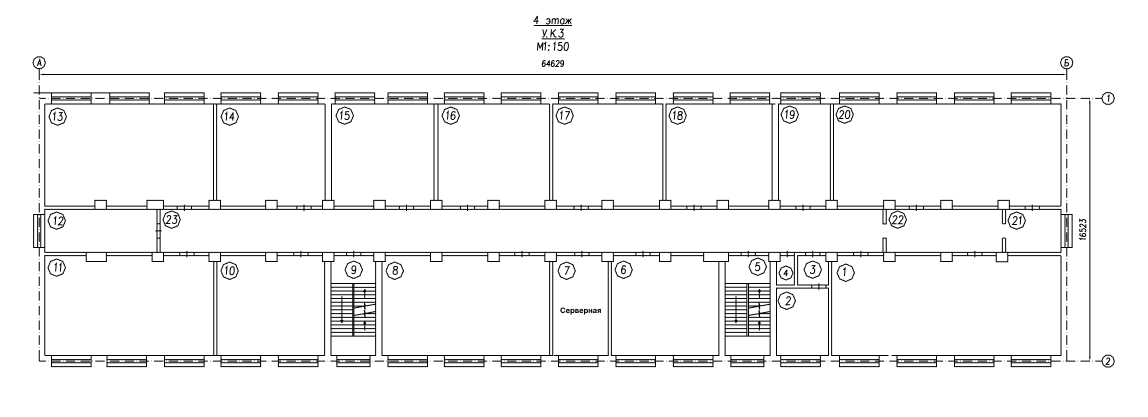
\includegraphics[width=180mm]{images/План объекта}
    \end{center}
    \captionsetup{justification=centering}
    \caption{План объекта}
    \label{fig::object_placement}
\end{figure}

\begin{longtable}{|p{5cm}|p{3cm}|p{8cm}|}
    \caption{Описание помещений на объекте}
    \label{tab::rooms_description} \\

    \hline
    Номер помещения &
    Площадь, м2 &
    Назначение \\
    \hline
    1 &
    96 &
    Учебное помещение \\
    \hline
    2 &
    14 &
    Служебное помещение \\
    \hline
    3 &
    3 &
    Служебное помещение \\
    \hline
    4 &
    2 &
    Служебное помещение \\
    \hline
    5 &
    - &
    Лестничная площадка \\
    \hline
    6 &
    44 &
    Учебное помещение \\
    \hline
    7 &
    22 &
    Серверная \\
    \hline
    8 &
    69 &
    Учебное помещение \\
    \hline
    9 &
    - &
    Лестничная площадка \\
    \hline
    10 &
    44 &
    Учебное помещение \\
    \hline
    11 &
    69 &
    Учебное помещение \\
    \hline
    12 &
    20 &
    Служебное помещение \\
    \hline
    13 &
    69 &
    Учебное помещение \\
    \hline
    14 &
    44 &
    Учебное помещение \\
    \hline
    15 &
    44 &
    Учебное помещение \\
    \hline
    16 &
    44 &
    Учебное помещение \\
    \hline
    17 &
    44 &
    Учебное помещение \\
    \hline
    18 &
    44 &
    Учебное помещение \\
    \hline
    19 &
    22 &
    Служебное помещение \\
    \hline
    20 &
    96 &
    Учебное помещение \\
    \hline
    21 &
    9 &
    Коридор \\
    \hline
    22 &
    20 &
    Коридор \\
    \hline
    23 &
    129 &
    Коридор \\
    \hline
\end{longtable}